\chapter{openPGP} \label{chapter:openpgp}

In this chapter we give an introduction into openPGP. We given an overview of the history and functionality. Furthermore we explain how this functionality is addressed by openPGP. In addition we list some common use-cases of openPGP implementations and compare openPGP with the related S/MIME protocol. 

% explain what it is, what it does and how it does it
% dont explain packet stuff in this chapter!

\section{History}  \label{section:openpgp:history}

In this section we give a short overview of the history of the openPGP standard and its most important implementations. \\


The Pretty Good Privacy (PGP) software was developed by Philip Zimmermann in 1991 \cite{PGP1} as a tool for human rights activists \cite{PGP2}. PGP was intended to be used to securely communicate via bulletin board systems, Usenet and E-Mail, but it can be used to encrypt and sign all kinds of data.

To allow interoperability with other programs the format used by PGP was standardized in 1997, forming the openPGP Message Format. \\


The openPGP standard is actively developed by the openPGP Working Group of the IETF. The WG was reopened in 2015 as reaction to an emerging discussion about secure (and usable) digital messaging.

\section{Functionality} \label{section:openpgp:functionality}

In this section we give an overview of the functionality provided by openPGP. We explain how openPGP provides confidentiality, integrity
and authentication. Furthermore we introduce openPGP's trust mode, the Web of Trust.  \\
% mention expire/revoke?
% mention passphrase?


Software based on the openPGP Message Format can be used to encrypt and decrypt data, as described in \cite[section 2]{RFC4880}. Furthermore it is possible to sign data and verify those signatures. In addition openPGP allows sender (and therefore message) authentication by defining its own trust model, called the Web of Trust. 

To do so openPGP combines asymmetric cryptosystems with symmetric cryptosystems. Asymmetric cryptosystems are used to provide message integrity by digitally signing data. Additionally they are used to exchange the keys used by symmetric cryptosystems. Symmetric cryptosystems are used to provide message confidentiality by encrypting data. OpenPGP allows the usage of various symmetric and asymmetric algorithms. \\


To provide this functionality every party participating in a communication secured by openPGP needs (at least) one openPGP key-pair. This key-pair consists of a public- and a private-key for usage by the asymmetric cryptosystem. A openPGP key is the composition of several cryptographic keys and meta-data. This composition is explained in detail in section \ref{section:messageformat:keys}. 


OpenPGP uses different keys for different functionality. For example it uses a different key-pair for digital signatures than for encryption. The signing-key-pair is used to provide integrity-protection and authentication of the key's meta-data. Furthermore it is the trust anchor in the Web of Trust. Therefore it is desired not to replace this key-pair. This is enabled by allowing replacement of the encryption-key-pair while keeping the signing-key-pair (and thus the trust on it).\\


\textbf{Message Confidentiality} is ensured by first encrypting data using a symmetric cipher using a session key generated randomly for every encryption, as described in \cite[section 2.1]{RFC4880}. The (symmetric) session key is then encrypted using the (asymmetric) public key of the receiver. The resulting encrypted session key is then prepended to the encrypted data and send to the receiver. The sender uses their (asymmetric) private key to decrypt the encrypted (symmetric) session key. The decrypted session key is then used to decrypt the actual data. This process is visualized in figure \ref{fig:encryption}.

If data is send to more than one receiver the (symmetric) session key is encrypted  multiple times using the public key of each receiver. The receiver then picks the encrypted session key encrypt to their key and decrypts it using their private key. Therefore it is not required to encrypt the data for each receiver separately.

In addition to the asymmetric key exchange it is possible to derive a symmetric key from a passphrase. In that case no asymmetric cryptosystem and therefore no key-pair is needed. This is useful if the data is stored and not transmited.\\

\textbf{Message Integrity} is provided by forming a digital signature of the (plaintext) data, as described in \cite[section 2.2]{RFC4880}. This is done by first calculating the hash of the data. Then the hash is signed using the private key of the sender. Afterward the calculated signature together with the encrypted data is send to the receiver. The receiver then uses their private key to encrypt the data. After that they are able to verify the integrity using the signature and the public key of the sender.

This system also allows non-repudiation, since signatures can only be issued by the holder of the private key.\\


To encrypt a message the openPGP public key of the designated receiver is needed. To verify the signature of a received message, the openPGP public key of the sender is needed, respectively. OpenPGP users therefore have to distribute their openPGP public keys. The easiest way to do perform this key-exchange is by sending the openPGP public key along with every message or by publishing it on a website. Another way to distribute openPGP public keys is by publishing them to a designated key directory, a so called key-server.


In the openPGP ecosystem it is assumed that it is not possible to transmit the openPGP public-key via a secure channel. Therefore it is necessary to validate the integrity and authenticity of a public-key before being able to use the key to validate the signature on a received message. It is necessary to validate this properties before encrypting to a public-key, respectively. In openPGP there are multiple ways to ensure \textbf{Sender Authentication}.

In the simplest case it is sufficient to hash the sensitive key-parts and then compare the hash-digest with the help of a secure channel (for example by phone or by printing it on a business card). In openPGP this hash over the public-key is called a fingerprint \cite[section 12]{RFC4880}.


In come cases it is not possible to compare this fingerprint, for example when the communication parties do not know each other in advance. In that case a more sophisticated approach is needed. For such cases openPGP provides its own trust model, called the \textbf{Web of Trust (WoT)} \cite{PGP2manual}. The WoT is a trust-model without any central authorities. Binding between the identity of an entity and a key-pair is done via cryptographic signatures. A user certifies (confirms) the authenticity of a keypair (its public key) by signing the identifying meta-data of the key with their own key. The resulting trust relation between the two keys is called certification. Since there exists no central certificate authority all openPGP users can issue certifications for all other openPGP keys. The result of this process is not a linear trust chain but a (directed) trust graph. \\

Sender authentication is created by searching for at least one (directed) patch from the sender's key-pair to the receiver's key-pair. A directed edge in the trust graph is represented by a digital signature. To establish a cryptographic trust path it is therefore needed to sign other openPGP keys. Since the owners of those keys signed other keys too it is possible to reach those keys by traversing on the edges. Thus it is possible to establish a trust path to before-unknown keys.

A detailed explanation of the Web of Trust approach and trust models in general was out of scope of this thesis. An analysis of the openPGP Web of Trust can be found in \cite{Ulrich2011}. \\


Because of the persistence (longevity) of a key-pair and the sensitivity of the private key it is necessary to be able to replace a key-pair or parts of it. Thus it is necessary to be able to invalidate the old key-pair. For this reasons openPGP provides the ability to set an \textbf{expiration date} for all public parts of an openPGP key-pair. In addition it is possible to \textbf{revoke} the key-pair or parts of it \cite[section 5.2]{RFC4880}. This is possible by adding a self-signature of a certain type to the openPGP key. This signals the invalidity to the openPGP implementation and requests not to use the specific key-part. \\

In addition openPGP provides funcitonality to protect private key material by encrypting it symmetrically using a passphrase \cite[section 3.7]{RFC4880}. Therefore this passphrase is required in addition to the private key file to decrypt or sign data.

\section{Applications} \label{section:openpgp:applications}

Although openPGP was designed to secure communication on bulletin boards it can be used in several different ways. In this section we given an overview of some of the possible applications. We explain how it can be used to secure email communication and what its limits are.  \\


In general terms software implementing the openPGP standard can be used to encrypt and sign data \cite[section 2]{RFC4880}. It does not limit the means of which the data has to be stored or transmitted. This allows to process generic files, for example to be securely stored on disk, transferred over the internet or printed on paper. In addition it is possible to use the \textit{Web of Trust} to authenticate entities. \\  


The main application of openPGP is to \textbf{secure email communication}. This can be achieved in two different ways. The more intuitive approach is to use a software implementing the openPGP standard to encrypt and sign the body and attachments of the message. After doing so the ciphertexts are put in place of the original data. The receive has to reverse that process by using a openPGP implementation to decrypt the message parts. This is possible without any changes to the email standard. The second approach uses an extension of the email standard called PGP/MIME \citep{RFC3156}. It utilizes special headers to structure the email data secured by openPGP.

Furthermore openPGP allows to only sign email messages without encrypting it \cite[section 7]{RFC4880}. This is also possible if the receiver is not using openPGP, resulting in the signature being displayed next to the message. This is an usability issue. To counteract this issue PGP/MIME hides the signature in its own email header. \\


The main limitation of both approaches is the fact that meta data is not signed \cite{Green2014}. In the email system it is not possible to protect the receiver of a message. In addition the email standard does not allow encryption or signing of the subject. \\

OpenPGP is also used to digitally \textbf{sign software}, a very common practice in the free/libre/open-source software (FLOSS) community. This is done to ensure integrity and authenticate the source of downloaded software. 

Because the community providing the software already build a Web of Trust it is easy to use openPGP. The used approach provides better security compared to unauthorized hashes. Furthermore it allows automated processing by package managers. \\

In addition it is possible to use openPGP keys for \textbf{Transport Layer Security} (TLS) authentication \cite{RFC6091}. This allows using a different trust model. Therefore it is possible to use the decentralized \textit{Web of Trust} instead of the hierarchical \textit{Public Key Infrastructure} \citep{RFC5280}. 

\section{Related protocol} \label{section:openpgp:smime}

In this section we give an overview of another protocol which provides the properties provided by openPGP. A short description of the Secure/Multipurpose Internet Mail Extensions (S/MIME) is given. Additionally the main differences between S/MIME and openPGP are highlighted. \\

The Secure/Multipurpose Internet Mail Extensions (S/MIME) \citep{RFC5751} is a standard for secure communication. It uses techniques similar to those used by openPGP to provide confidentiality, message integrity and sender authentication. S/MIME was designed to secure email communication.  \\

The main differences between openPGP and S/MIME is the structure of the used trust model.  \\

The \textbf{OpenPGP} protocol provides sender and key authentication via a decentralized trust mode. It uses a \textit{Web of Trust} to bind the identity of an entity to a key. This allows a trust model without any central authority. Every user of openPGP is able to issue a trust certification for every other openPGP key. This model is explained in section \ref{section:openpgp:functionality}. The downside of this approach is a lack of usability. To securely authenticate a key it is required to find a cryptographic trust path to the receiver's key. Another issue is that it is not defined what the meaning of an openPGP certification is. Every user decides for themselves about the requirements for a certification. The topic of usability is further discussed in chapter \ref{section:concerns:usability}. \\

In contrast to this the \textbf{Secure/Multipurpose Internet Mail Extensions (S/MIME)} \citep{RFC5751} standard provides sender authentication by setting up a tree-like trust hierarchy. S/MIME uses the \textit{X.509 public key infrastructure (PKI)} \citep{RFC5280} as trust model. Trust is issued by central Certificate Authorities (CAs). A CA uses their private key to digitally sign the receiver's key. The resulting signature is called a certificate. To authenticate a key it is required to find a cryptographic trust path from a trusted CA to the receiver's key. There are multiple ways to ensure if a CA is trusted. One was is to install the CA's certificate (containing its public key) on the receiver's system. This can be done by operating-system or browser vendors, IT departments or manually by the user. This CAs are called \textit{root CA}. Another way to ensure trust in the CA is to sign the CA's certificate itself. This creates a trust hierarchy. \\

Figure \ref{fig:pkiwot} shows the difference in terms of structure of the two mentioned trust models.

\begin{figure}
	\centering
	\begin{subfigure}{.5\textwidth}
		\centering
		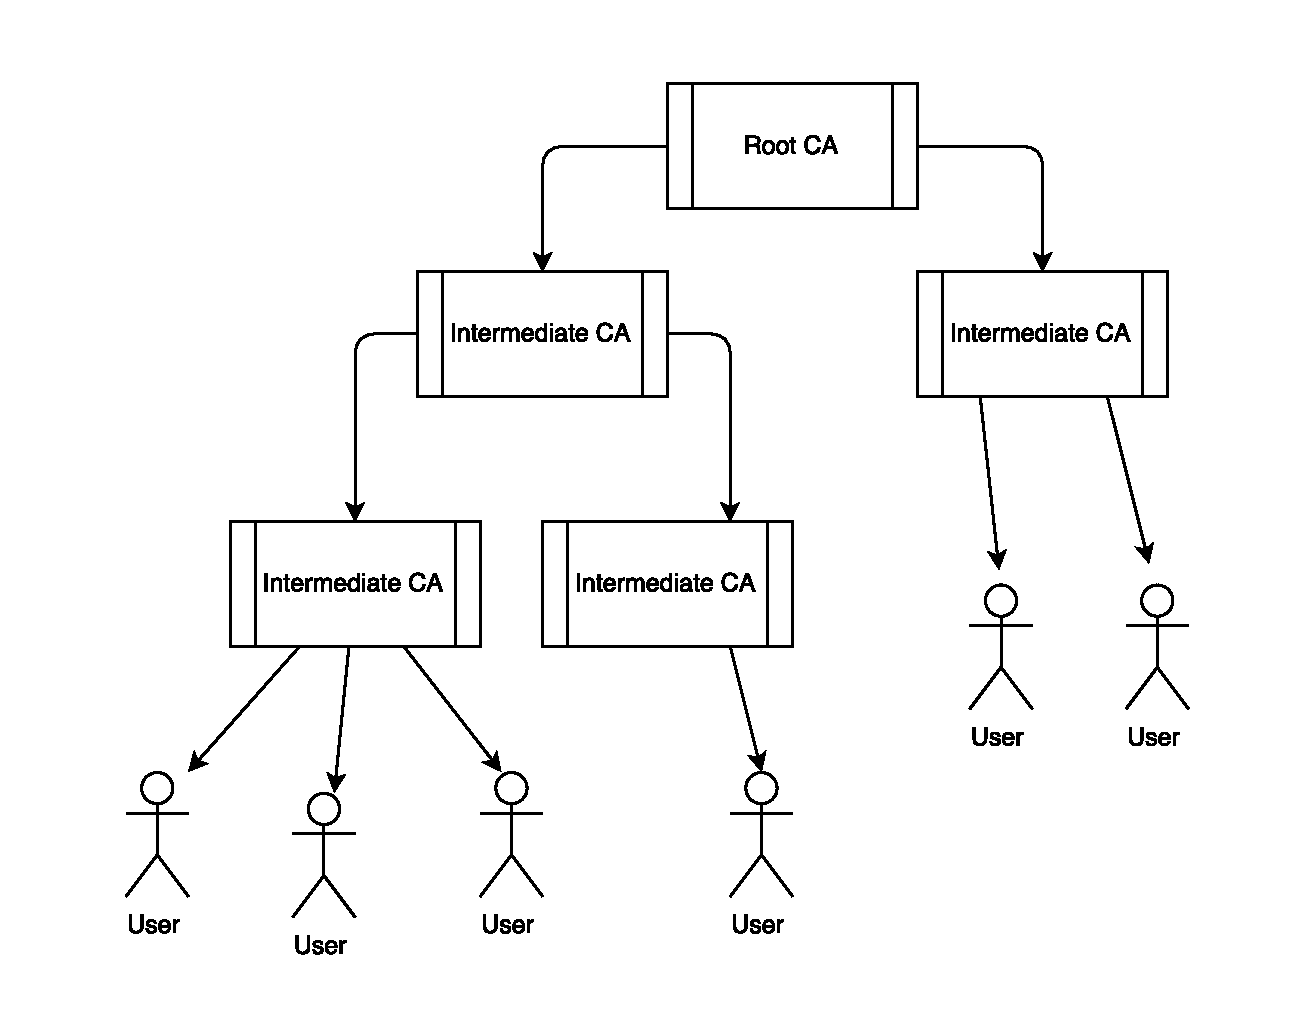
\includegraphics[width=1\linewidth]{figures/PKI}
		\caption{Public Key Infrastructure (PKI)}
		\label{fig:pki}
	\end{subfigure}%
	\begin{subfigure}{.5\textwidth}
		\centering
		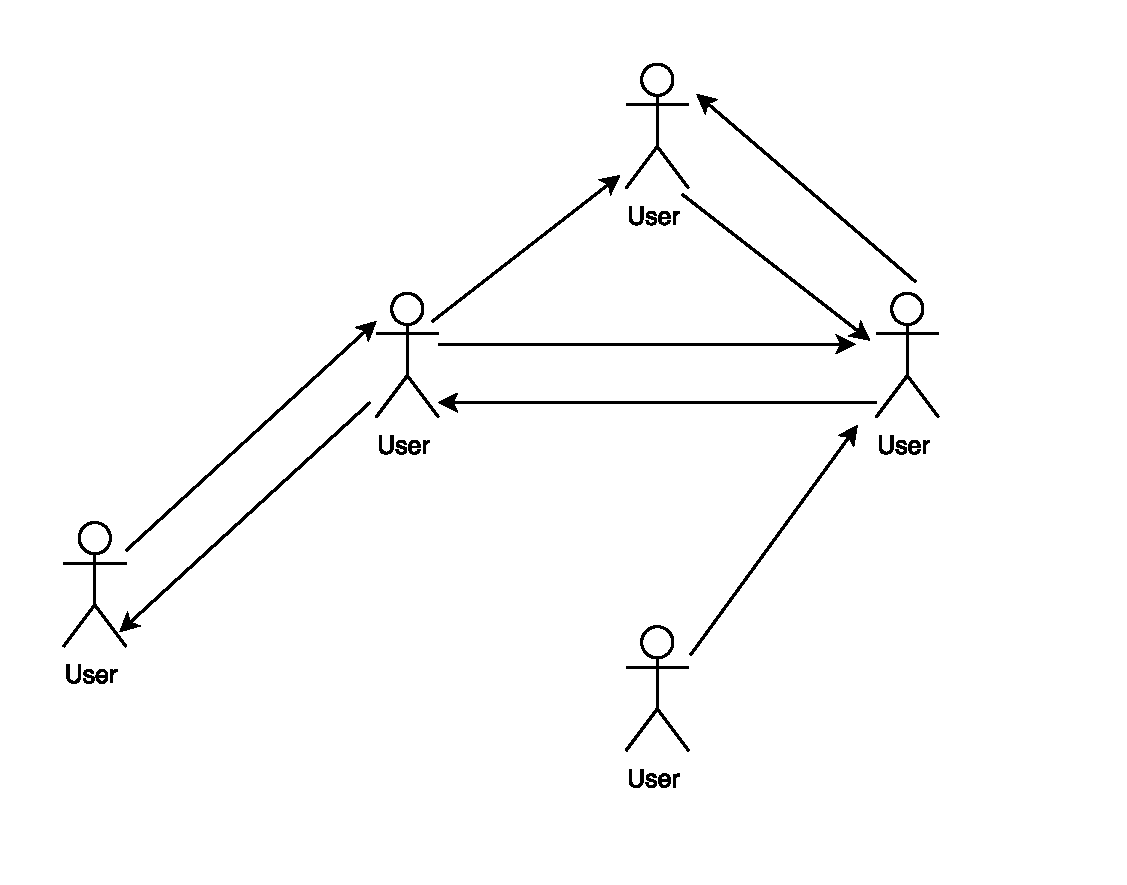
\includegraphics[width=1\linewidth]{figures/WOT}
		\caption{Web of Trust (WOT)}
		\label{fig:wot}
	\end{subfigure}
	\caption{Comparison of PKI and WoT}
	\label{fig:pkiwot}
\end{figure}


